\documentclass[12pt]{article}
\usepackage[utf8]{inputenc}
\usepackage{textcomp}
\usepackage{graphicx}
\usepackage{amsmath}
\usepackage{siunitx}
\usepackage{booktabs}
\usepackage{textalpha}
\usepackage{float}
\usepackage{geometry}
\usepackage[portuguese]{babel}

\geometry{
 a4paper,
 left=3cm,
 top=2cm,
 right=2cm,
 bottom=2cm
}

\begin{document}

\begin{center}
    \textbf{\large UNIVERSIDADE FEDERAL DO RIO GRANDE DO SUL} \\
    \textbf{\large INSTITUTO DE FÍSICA} \\
    \vspace{3cm}
    \textbf{\Large CADERNO DE LABORATÓRIO 1} \\
    \vspace{1cm}
    \textbf{\large DETERMINAÇÃO DA RESISTÊNCIA DE UM RESISTOR} \\
    \vspace{3cm}
    
    \begin{tabular}{rl}
        \textbf{Integrantes:} & Guilherme Franke Riter - 00579589 \\
                               & Júlia Matzenbacher Henicka Germano - 00579271 \\
                               & Leonardo Kawai Suarez - 00578511 \\
                               & Leonardo Werner Morel Dias - 00590887 \\
    \end{tabular}
    
    \vspace{12cm}
    \textbf{\large Porto Alegre, RS} \\
    \textbf{\large 30 de abril de 2025} \\ % Data atual (pode substituir por uma data fixa se preferir)
\end{center}\newpage

\section*{Parte A: Determinação pelo Código de Cores}

Identificamos as faixas coloridas no resistor e consultamos a tabela de código de cores.

\begin{itemize}
    \item Sequência de cores: Marrom - Preto - Vermelho - Dourado
    \item Valor nominal: \( R_{\text{nominal}} = \SI{1000}{\ohm} \)
    \item Tolerância percentual: \( \pm 5\% \)
    \item Tolerância absoluta: \( \pm \SI{50}{\ohm} \)
    \item Faixa de valores esperados:
    \begin{itemize}
        \item \( R_{\text{min}} = \SI{950}{\ohm} \)
        \item \( R_{\text{max}} = \SI{1050}{\ohm} \)
    \end{itemize}
\end{itemize}

\section*{Parte B: Medição Direta com Ohmímetro}

Medição direta com multímetro digital na função ohmímetro.

\begin{itemize}
    \item Valor medido: \(R_{med} = \SI{995}{\ohm} \)
    \item Incerteza: \(\sigma_{med} = \pm \SI{10}{\ohm} \)
    \item Resultado: \(R_{med} = \SI{995}{\ohm} \pm \num{10} \, \si{\ohm} \)
\end{itemize}

\section*{Parte C: Método Indireto Rápido}

O circuito foi montado conforme o esquema abaixo:
\begin{figure}[H]
    \centering
    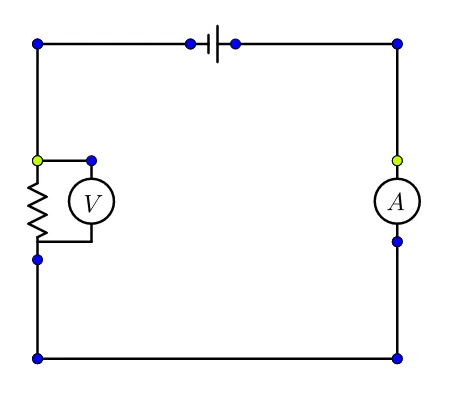
\includegraphics[width=0.5\textwidth]{circuito-lab1.png}
    \caption{Esquema do circuito montado.}
    \label{fig:circuito}
\end{figure}

\begin{itemize}
    \item Valores medidos:
    \begin{itemize}
        \item \( I = \SI{5.37}{\milli\ampere} \pm \SI{0.05}{\milli\ampere} \)
        \item \( V_R = \SI{5.18}{\volt} \pm \SI{0.01}{\volt} \)
    \end{itemize}
    \item Resistência calculada: \(R_{ind} = \SI{965}{\ohm}\)
    \item Incerteza propagada: \begin{equation}
        \sigma_{ind} = \sqrt{\sigma_{I}^2+\sigma_{V_R}^2} = \sqrt{(\sqrt{(0.01\cdot5.37)^2 + (0.01)^2})+(\sqrt{(0.008\cdot5.18)^2 + (0.01)^2})} = \SI{9}{\ohm}
    \end{equation}
    
    \item Resultado: \(R_{ind} = \SI{965}{\ohm} \pm \num{9} \, \si{\ohm} \)
\end{itemize}

\section*{Parte D: Análise do Gráfico \( V \times I \)}

\subsection*{Cálculo das Incertezas}

A partir dos dados coletados em laboratório e das informações disponíveis no manual técnico do multímetro, calculamos as incertezas associadas à resolução e à precisão do equipamento, conforme código abaixo, implementado no software Scilab.

\begin{verbatim}
// Cálculo das incertezas para tensão (V)
delta_V = zeros(n, 1);
for i = 1:n
    if V(i) < 0.4 then
        delta_V(i) = sqrt((0.016*V(i))^2 + (0.0001)^2);
    elseif V(i) < 4 then
        delta_V(i) = sqrt((0.008*V(i))^2 + (0.001)^2);
    elseif V(i) < 40 then
        delta_V(i) = sqrt((0.008*V(i))^2 + (0.01)^2);
    elseif V(i) < 400 then
        delta_V(i) = sqrt((0.008*V(i))^2 + (0.1)^2);
    else
        delta_V(i) = sqrt((0.01*V(i))^2 + (1)^2);
    end
end

// Cálculo das incertezas para corrente (mA)
delta_I = zeros(n, 1);
for i = 1:n
    if I(i) < 0.4 then
        delta_I(i) = sqrt((0.01*I(i))^2 + (0.0001)^2);
    elseif I(i) < 4 then
        delta_I(i) = sqrt((0.01*I(i))^2 + (0.001)^2);
    elseif I(i) < 40 then
        delta_I(i) = sqrt((0.01*I(i))^2 + (0.01)^2);
    elseif I(i) < 400 then
        delta_I(i) = sqrt((0.01*I(i))^2 + (0.1)^2);
    else
        delta_I(i) = sqrt((0.012*I(i))^2 + (1)^2);
    end
end
\end{verbatim}

Com isso, obtemos a seguinte tabela de dados:

\begin{table}[H]
\centering
\caption{Dados experimentais de tensão (V) e corrente (I) com incertezas.}
\label{tab:dados_experimentais}
\begin{tabular}{cccc}
\toprule
\textbf{$V$ (V)} & \textbf{$\Delta V$ (V)} & \textbf{$I$ (mA)} & \textbf{$\Delta I$ (mA)} \\ 
\midrule
0.119  & 0.0019 & 0.110  & 0.0011 \\ 
1.680  & 0.0135 & 1.720  & 0.0172 \\ 
2.640  & 0.0211 & 2.720  & 0.0272 \\ 
3.300  & 0.0264 & 3.390  & 0.0339 \\ 
4.330  & 0.0361 & 4.450  & 0.0456 \\ 
5.180  & 0.0426 & 5.370  & 0.0546 \\ 
6.090  & 0.0497 & 6.300  & 0.0638 \\ 
6.990  & 0.0568 & 7.240  & 0.0731 \\ 
7.990  & 0.0647 & 8.290  & 0.0835 \\ 
8.940  & 0.0722 & 9.290  & 0.0934 \\ 
\bottomrule
\end{tabular}
\end{table}

\subsection*{Ajuste Linear}

Da tabela acima, realizamos um ajuste linear rápido utilizando o software SciDavis, cujos resultados são apresentados na tabela a seguir:

\begin{table}[H]
\centering
\caption{Resultados detalhados do ajuste linear.}
\label{tab:ajuste_detalhado}
\begin{tabular}{ll}
\toprule
\textbf{Item} & \textbf{Descrição} \\
\midrule
Função & $I = (1.0359 \pm 0.0036)V - (0.0133 \pm 0.0012)$ \\
Intervalo & $V \in [0.119,\, 8.94]$ V \\
Qualidade & $\chi^2 = 1.0465$ \quad $R^2 = 0.999987$ \\
Incertezas & Baseadas na Tabela 1 \\
\bottomrule
\end{tabular}
\end{table}

Então, a curva de ajuste linear, de forma \( I = aV + b \), é dada por:

\begin{equation}
    I = (1.0359 \pm 0.0036)V - (0.0133 \pm 0.0012)
\end{equation}

\begin{figure}[H]
    \centering
    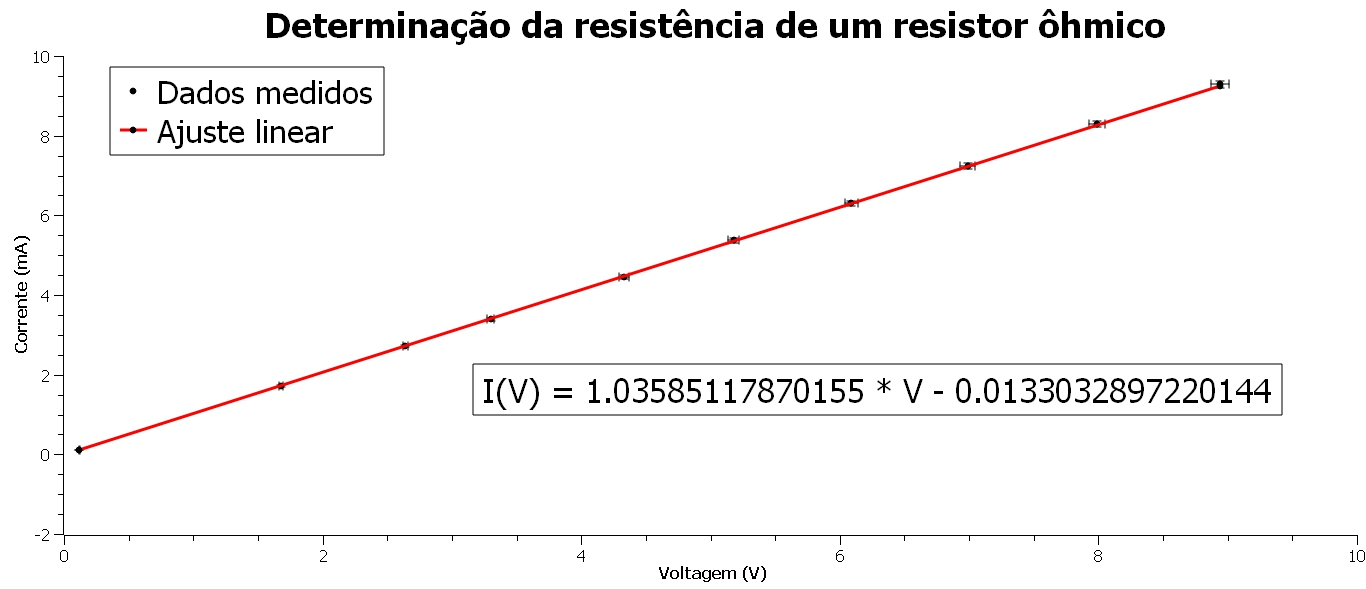
\includegraphics[width=\textwidth]{grafico-lab1.jpeg}
    \caption{Gráfico de \( V \) versus \( I \) com ajuste linear.}
    \label{fig:ajuste_linear}
\end{figure}

Do gráfico acima, verificamos que a relação entre \( V \) e \( I \) é linear, confirmando o comportamento ôhmico do resistor. Os valores de \(\chi^2\) e \(R^2\) indicam um bom ajuste, com \(R^2\) próximo de 1, o que sugere que a maioria dos dados se ajusta bem à reta.

Para calcular a resistência do resistor, primeiro notamos que a declividade da reta é dada por \( a = \frac{1}{R} \), onde \( R \) é a resistência do resistor. Assim, podemos encontrar o valor de \( R \) a partir da declividade:

\begin{equation}
    R = \frac{1}{a} = \frac{1}{(1.0359 \pm 0.0036)} = (963.6 \pm 3.4) \, \si{\ohm}
\end{equation}

\subsection*{Análise dos Valores Obtidos}
Todos os métodos apresentaram resultados consistentes dentro das faixas de incerteza:
\begin{itemize}
    \item \textbf{Código de cores} (1000 ± 50 Ω): Valor nominal dentro da tolerância esperada.
    \item \textbf{Medição direta} (995 ± 10 Ω): Resultado mais próximo do nominal com baixa incerteza.
    \item \textbf{Método indireto} (965 ± 9 Ω): Valor ligeiramente abaixo, porém dentro da faixa aceitável.
    \item \textbf{Ajuste gráfico} (963.6 ± 3.4 Ω): Valor mais preciso, com incerteza reduzida.
\end{itemize}

\subsection*{Comparação dos Métodos}

\begin{table}[H]
    \centering
    \begin{tabular}{@{}llll@{}}
        \toprule
        \textbf{Método} & \textbf{Vantagens} & \textbf{Desvantagens} & \textbf{Aplicação Ideal} \\
        \midrule
        Código de cores & 
        \begin{minipage}[t]{0.2\textwidth}
            \begin{itemize}
                \item Rápido
                \item Não requer instrumentos
            \end{itemize}
        \end{minipage} &
        \begin{minipage}[t]{0.25\textwidth}
            \begin{itemize}
                \item Incerteza alta (5\%)
                \item Subjetivo
            \end{itemize}
        \end{minipage} &
        Verificação inicial \\
        
        Medição direta & 
        \begin{minipage}[t]{0.2\textwidth}
            \begin{itemize}
                \item Simples
                \item Baixa incerteza
            \end{itemize}
        \end{minipage} &
        \begin{minipage}[t]{0.25\textwidth}
            \begin{itemize}
                \item Requer equipamento
                \item Limitação de faixa
            \end{itemize}
        \end{minipage} &
        Medições rápidas \\
        
        Método indireto & 
        \begin{minipage}[t]{0.2\textwidth}
            \begin{itemize}
                \item Verifica Lei de Ohm
                \item Versátil
            \end{itemize}
        \end{minipage} &
        \begin{minipage}[t]{0.25\textwidth}
            \begin{itemize}
                \item Erros sistemáticos
                \item Mais complexo
            \end{itemize}
        \end{minipage} &
        Circuitos simples \\
        
        Ajuste gráfico & 
        \begin{minipage}[t]{0.2\textwidth}
            \begin{itemize}
                \item Menor incerteza
                \item Análise estatística
            \end{itemize}
        \end{minipage} &
        \begin{minipage}[t]{0.25\textwidth}
            \begin{itemize}
                \item Complexo
                \item Requer software
            \end{itemize}
        \end{minipage} &
        Precisão máxima \\
        \bottomrule
    \end{tabular}
    \caption{Comparação detalhada dos métodos de medição}
\end{table}

\end{document}